\documentclass[UTF8]{ctexart}
\usepackage{mathtools,wallpaper}

\usepackage{t1enc}
\usepackage{pagecolor}
\usepackage{geometry}
\usepackage{diagbox}
\usepackage{graphicx}
\usepackage{wrapfig}
\usepackage{amssymb}

\geometry{left=2cm,right=2cm}

\begin{document}

\CTEXsetup[format={\Large\bfseries}]{section}
\title{实验报告}  
\author{徐亦昶 PB20000156}
\maketitle
\section{实验题目}分光计B
\section{实验目的}
\begin{enumerate}
    \item 掌握分光计的原理和使用方法
    \item 利用分光计测量三棱镜的折射率
\end{enumerate}
\section{实验原理}
\subsection{分光计的结构}
分光计的外形如图所示。
\begin{figure}[h]
    \centering
    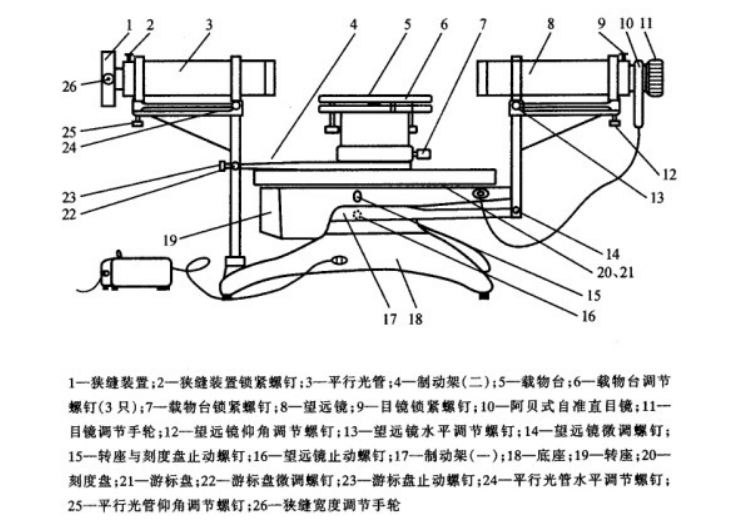
\includegraphics[scale=1]{分光计外形图.PNG}
    \caption{分光计外形图}
\end{figure}
重点解释望远镜和读数圆盘:
\begin{enumerate}
    \item 望远镜:由目镜系统和物镜组成,目镜和物镜之间装有分划板,它们分
    别置于内管、外管和中管内,三个管彼此可以相互移动,也可以用螺钉固定。
    在中管的分划板下方紧贴一块$45^o$全反射小棱镜,棱镜与分划板的粘贴部分涂成
    黑色,仅留一个绿色的小十字窗口。光线从小棱镜的另一直角边入射,从$45^o$反射面
    反射到分划板上,透光部分便形成一个在分划板上的明亮的十字窗。
    \item 读数圆盘:由刻度盘和游标盘组成。刻度盘上由720等分刻线,格值为0.5度。游标盘
    上有两个游标,互为对径点,最小分度为1'。读数时,要读出两个游标处的读数值,然后取
    平均值,这样可消除刻度盘和游标盘的圆心与仪器主轴的轴心不重合所引起的偏心误差。
\end{enumerate}
\subsection{分光计的调整原理和方法}
实验开始前,要先调整分光计使得平行光管发出平行光,望远镜对平行光聚焦,且望远镜、平行光管的光轴垂直仪器公共轴。
具体有如下几步。
\subsubsection{目镜调焦}
旋转调焦手轮,使得目镜中显示的分划板刻线清晰。
\subsubsection{调望远镜对平行光聚焦}
\begin{enumerate}
    \item 将反射镜放到载物台上,使得一端正对某个调节螺钉。\
    \item 用眼睛观测,粗调望远镜光轴与镜面垂直。
    \item 沿轴向移动目镜筒,使得目镜中看到的绿十字清晰。
\end{enumerate}
\subsubsection{调整望远镜光轴垂直仪器主光轴}
使用折半调整法(即每次目镜和载物台各调一半),使得在载物台正常、旋转180度、旋转120度时绿十字分划板
上与下方十字窗对称的上十字线中心。
\subsubsection{调整平行光管发出平行光并垂直仪器主轴}
\begin{enumerate}
    \item 取下平面镜和目镜照明光源,狭缝对准前方汞灯光源,使望远镜转向平行光管方向,在目镜中
    观察狭缝像,沿轴向移动狭缝筒,直到像清晰。
    \item 将狭缝转向横向,调螺钉(25),将像调到中心横线上。这表明平行光管光轴已与望远镜
    光轴共线,所以也垂直仪器主轴。螺钉(25)不能再动。
    \item 将狭缝调成垂直,锁紧螺钉。
\end{enumerate}
\subsection{用最小偏向角法测三棱镜材料的折射率}
\begin{figure}[h]
    \centering
    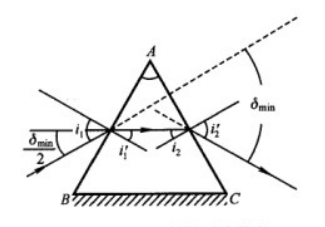
\includegraphics[scale=1]{折射率测量原理.PNG}
    \caption{三棱镜最小偏向角原理图}
\end{figure}
从图中可以看出,
\[i_1'=\frac{A}{2},\]
\[\frac{\delta_{min}}{2}=i_1-i_1'=i_1-\frac{A}{2},\]
\[i_1=\frac{1}{2}\left( \delta_{min}+A \right).\]
设棱镜材料折射率为n,则
\[sin i_1=nsin i_1'=nsin\frac{A}{2}\]
故
\[n=\frac{sin i_1}{sin\frac{A}{2}}=\frac{sin\frac{\delta_{min}+A}{2}}{sin \frac{A}{2}}\]
于是,要测折射率n,只需测出其顶角A和最小偏向角$\delta_{min}$。
\section{实验内容}
先参照原理部分叙述的方法调整分光计。
\subsection{使三棱镜光学侧面垂直望远镜光轴}
\begin{enumerate}
    \item 调载物台的上下台面大致平行,将棱镜放到平台上,使棱镜三边与台下三螺钉的连线所成三边相互垂直。
    \item 转动载物台,使得可以从望远镜中看到反射回来的十字像;只调台下三螺钉,使反射的绿十字像落到上十字线上。
\end{enumerate}
\subsection{测棱镜顶角}
\begin{enumerate}
    \item 旋紧度盘下螺钉,使望远镜和刻度盘固定不动。
    \item 设棱镜为ABC,先使AC面正对望远镜,记下游标1的读数$\theta_1$和游标2的读数$\theta_2$。
    \item 转动游标盘,使AB面正对望远镜,记下游标1的读数$\theta_1'$和游标2的读数$\theta_2'$。
    \item 计算$A=\pi-\frac{1}{2}\left[ | \theta_1-\theta_1'| +| \theta_2-\theta_2'|  \right]$。
\end{enumerate}
\subsection{测三棱镜的最小偏向角}
\begin{enumerate}
    \item 平行光管狭缝对准前方汞灯光源。
    \item 旋松望远镜止动螺钉(16)和游标盘止动螺钉(23),旋转载物台和望远镜,使得望远镜中可以看见汞灯光谱线
    \item 轻轻转动载物台,使谱线往$\delta$减小的方向移动,并让望远镜跟踪光谱移动,知道棱镜停止转动,而谱线开始要反方向移动。
    \item 固定载物台,再使望远镜微动,使其分划板上的中心竖线对准其中的那条绿谱线。
    \item 使用与测量顶角类似的方法测量。此时最小偏向角的计算公式为$\delta_{min}=\frac{1}{2}\left[ | \theta_1-\theta_1'| +| \theta_2-\theta_2'|  \right]$。
    \item 计算折射率n及其不确定度。
\end{enumerate}
\section{数据记录}
\begin{table*}[htbp]
    \centering
    \fontsize{8}{10}\selectfont
    \caption{顶角测量}
    \scalebox{1.15}{
    \begin{tabular}{|c|c|c|c|}
    \hline
    $\theta_1$ & $\theta_2$ & $\theta_1'$ & $\theta_2'$ \\
    \hline
     $14^o8'$ & $194^o12'$ & $134^o10'$ & $314^o5'$\\
     \hline
     $25^o2'$ & $205^o3'$ & $145^o25'$ & $325^o32'$\\
     \hline
     $50^o13'$ & $230^o15'$ & $270^o40'$ & $350^o20'$\\
     \hline
    \end{tabular}}
\end{table*}
\begin{table*}[htbp]
    \centering
    \fontsize{8}{10}\selectfont
    \caption{最小偏向角测量}
    \scalebox{1.15}{
    \begin{tabular}{|c|c|c|c|}
    \hline
    $\theta_1$ & $\theta_2$ & $\theta_1'$ & $\theta_2'$ \\
    \hline
     $104^o20'$ & $284^o22'$ & $49^o1'$ & $229^o2'$\\
     \hline
     $80^o5'$ & $260^o14'$ & $135^o26'$ & $315^o23'$\\
     \hline
     $13^o41'$ & $193^o17'$ & $68^o24'$ & $248^o26'$\\
     \hline
    \end{tabular}}
\end{table*}
\cite{chen2020tois}
\section{数据计算}
\subsection{顶角测量}
根据$A=\pi-\frac{1}{2}\left[ | \theta_1-\theta_1'| +| \theta_2-\theta_2'|  \right]$,
计算出3次测量所得的A分别为$59^o56',59^o34',55^o46'$,求平均值,得$A=59^o45'$
\subsection{最小偏向角测量}
根据$\delta_{min}=\frac{1}{2}\left[ | \theta_1-\theta_1'| +| \theta_2-\theta_2'|  \right]$,
可算出三次测量得到的最小偏向角分别为$55^o20',55^o15',55^o13'$,因此取平均后为$55^o16$。
\subsection{折射率计算}
\[n=\frac{sin\frac{\delta_{min}+A}{2}}{sin \frac{A}{2}}=1.69\]
\section{不确定度分析}
先考虑顶角A。
$A$的A类不确定度
$u_{1A}=\sqrt{\frac{\Sigma_{i=1}^3(A_i-\overline{A})^2}{3\times \left( 3-1 \right))}}=6.36'$。当置信概率P=0.95时,t因子
$t_{0.95}=2.26$。游标盘最大允差1',估计误差可忽略不计(比仪器误差小得多)。
因此$\Delta_B=1'$。由于所用仪器符合正态分布,所以C=3,且$t_P=1.96$,所以
B类不确定度$u_B=\frac{\Delta_B}{C}=0.3'$。
所以合成不确定度$U_{0.95}=\sqrt{\left( t_{0.95}\cdot u_A \right)^2+\left( t_P\cdot u_B \right)^2}=14'$
\newline
再考虑最小偏向角$\delta_{min}$。
$A$的A类不确定度
$u_{2A}=\sqrt{\frac{\Sigma_{i=1}^3(\delta_i-\overline{\delta})^2}{3\times \left( 3-1 \right))}}=2.08'$。当置信概率P=0.95时,t因子
$t_{0.95}=2.26$。游标盘最大允差1',估计误差可忽略不计(比仪器误差小得多)。
因此$\Delta_B=1'$。由于所用仪器符合正态分布,所以C=3,且$t_P=1.96$,所以
B类不确定度$u_B=\frac{\Delta_B}{C}=0.3'$。
所以合成不确定度$U_{0.95}=\sqrt{\left( t_{0.95}\cdot u_A \right)^2+\left( t_P\cdot u_B \right)^2}=5'$
\newline
最后计算n的不确定度。
根据不确定度传递公式
\[U_n^2=(\frac{sin\frac{\delta_{min}}{2}}{2sin^2\frac{A}{2}})^2U_A^2+(\frac{sin\frac{\delta_{min}}{2}}{2}-\frac{cos\frac{\delta_{min}}{2}cot\frac{A}{2}}{2}-\frac{1}{2}sin\frac{\delta_{min}}{2})^2U_{\delta_{min}}^2=0.03\]
因此折射率为$n=1.69\pm 0.03$。
\section{思考}
因为载物台的表面没有平行于度盘,将平面镜取下后,又放到载物台上(放的位置与拿下前的位置不同),这时平面
镜法线已经不与仪器主轴垂直了,所以反射镜两个面的反射像的位置就不正确了。不能说明望远镜光轴还没有调好。
\end{document}